%%% spell check: aug 29, 2014
%%%% handouts:  pdfjam --landscape --nup '2x2' ecology4.pdf
%%%% handouts:  pdfjam --landscape ecology4.pdf

%\documentclass[handout]{beamer}
\documentclass[10pt]{beamer}

\usepackage{parskip}
\setlength{\parskip}{1.75ex}

\mode<presentation>
{\usetheme{Singapore}
\setbeamercovered{transparent}}

\title{R Minicourse Workshop, Part 4}

\author{\small Presented to the\\
        Washington State Deptment of Ecology\\
       September 2--3, 2014}

\date{\scriptsize Dr.~Robin Matthews, Institute for Watershed Studies\\
   Dr. Geoffrey Matthews, Computer Science Department\\
   Western Washington University}


\setbeamertemplate{blocks}[rounded][shadow=true]
\setbeamertemplate{footline}{\hspace*{5ex}Part 4 - Sept.~3, 2014 
   \hfill Page \insertframenumber \hspace{0.1ex} of
   \inserttotalframenumber \hspace*{5ex}
   \vspace*{2ex}}

\begin{document}
\lecture{R Minicourse}{Section 4}
\newcommand{\be}{\begin{enumerate}}
\newcommand{\ee}{\end{enumerate}}
\newcommand{\bi}{\begin{itemize}}
\newcommand{\ei}{\end{itemize}}
\newcommand{\bd}{\begin{description}}
\newcommand{\ed}{\end{description}}


\begin{frame}
\titlepage
\end{frame}

\begin{frame}
\frametitle{Introduction to Multivariate Analysis}
\framesubtitle{Initial Examination of Multivariate Data}

\bi
\item Begin by plotting and using simple exploratory tools like 
  analysis to look for patterns
\bi
\item Don't use complicated multivariate tests to describe
  simple univariate or bivariate patterns
\ei

\item Check for normality and homoscedasticity  $\ldots$ nearly all
  multivariate methods are sensitive to heteroscedastic variances

\item Identify redundant, nonlinear, and random variables
\bi
\item 
Including redundant, nonlinear, and random variables in
  multivariate analysis can obscure patterns in the remaining variables
\ei
\item Identify variables with {\em zero} variance (all samples have same value)
\bi
\item This type of response isn't useful in multivariate analysis
\ei
\ei
\end{frame}

\begin{frame}
\frametitle{Introduction to Multivariate Analysis, Continued}

\bi
\item Most multivariate methods involve reorganizing the data matrix
  to find linear or monotonic patterns, or simplifying a complex data
  sets to identify a subset of variables that best describe the
  patterns in the data

   \bi
   \item Not all multivariate patterns will be linear or monotonic!

    \item Multivariate patterns can be significant even if the individual
    univariate patterns are not significant
   \ei

\item 
Two common multivariate patterns include similarity among groups of
samples (clustering) and increasing dissimilarity along a gradient
(ordination)

\ei

\end{frame}



\begin{frame}
\frametitle{Introduction to Multivariate Analysis}
\framesubtitle{Clustering vs.~Ordination}

{\footnotesize
{\color{blue}Clustering} involves finding similarity among groups of samples:

\begin{center}
\begin{tabular}{|cccccc||cccccc|} \hline
A & B & C & D & E & F	& E & C & A & D & F & B\\ \hline
2 & 3 & 1 & 2 & 1 & 3	& {\color{red}1} & {\color{red}1} & {\color{blue}2} & {\color{blue}2} & {\color{green}3} & {\color{green}3}\\
2 & 3 & 1 & 2 & 1 & 3	& {\color{red}1} & {\color{red}1} & {\color{blue}2} & {\color{blue}2} & {\color{green}3} & {\color{green}3}\\
3 & 1 & 2 & 3 & 2 & 1	& {\color{red}2} & {\color{red}2} & {\color{blue}3} & {\color{blue}3} & {\color{green}1} & {\color{green}1}\\
3 & 1 & 2 & 3 & 2 & 1	& {\color{red}2} & {\color{red}2} & {\color{blue}3} & {\color{blue}3} & {\color{green}1} & {\color{green}1}\\
1 & 2 & 3 & 1 & 3 & 2	& {\color{red}3} & {\color{red}3} & {\color{blue}1} & {\color{blue}1} & {\color{green}2} & {\color{green}2}\\
1 & 2 & 3 & 1 & 3 & 2	& {\color{red}3} & {\color{red}3} & {\color{blue}1} & {\color{blue}1} & {\color{green}2} & {\color{green}2}\\ \hline
\end{tabular}
\end{center}


{\color{blue}Ordination} looks for increasing dissimilarity along a gradient:

\begin{center}
\begin{tabular}{|cccccc||cccccc|} \hline
A & B & C & D & E & F	& E & C & A & D & F & B\\ \hline
3 & 6 & 2 & 4 & 1 & 5	& {\color{red}1} & {\color{blue}2} & {\color{green}3} & 4 & {\color{green}5} & {\color{blue}6}\\
2 & 5 & 1 & 3 & 6 & 4	& {\color{blue}6} & {\color{red}1} & {\color{blue}2} & {\color{green}3} & 4 & {\color{green}5}\\
1 & 4 & 6 & 2 & 5 & 3	& {\color{green}5} & {\color{blue}6} & {\color{red}1} & {\color{blue}2} & {\color{green}3} & 4\\
6 & 3 & 5 & 1 & 4 & 2	& 4 & {\color{green}5} & {\color{blue}6} & {\color{red}1} & {\color{blue}2} & {\color{green}3}\\
5 & 2 & 4 & 6 & 3 & 1	& {\color{green}3} & 4 & {\color{green}5} & {\color{blue}6} & {\color{red}1} & {\color{blue}2}\\
4 & 1 & 3 & 5 & 2 & 6	& {\color{blue}2} & {\color{green}3} & 4 & {\color{green}5} & {\color{blue}6} & {\color{red}1}\\ \hline
\end{tabular}
\end{center}
}

\end{frame}




\begin{frame}
\frametitle{Multivariate Ordination}
\framesubtitle{Principal Components Analysis}

\bi
\item PCA is a linear model that searches for combinations of
variables that explain the most variance in the data

\item Because PCA is a linear model, it is influenced by
all problems affecting regression/correlation

\item PCA uses {\em all variables}, so random variables can be
  a problem

\item PCA uses combinations of variables, so multivariate
  homoscedasticity is important

\bi
\item Most PCA applications are {\em row centered} and {\em
  standardized}, which converts from a co-variance PCA to a correlation PCA
\ei

\ei
\end{frame}

%%%% Kaiser's criterion:  keep components with variance above 1;
%%%% results in about same as keeping components above ``elbow'' in var plot


\begin{frame}[fragile]
\frametitle{Principal Components Analysis} 
\framesubtitle{{\tt \color{red} R} Syntax Using {\color{red} \tt
    prcomp} and {\color{red} \tt princomp}}

\bi
\item There are two basic PCA methods: {\color{red} \tt princomp} and
  {\color{red} \tt prcomp}

   \bi
   \item {\color{red} \tt princomp} ordinated using an eigenvalue matrix
   \item {\color{red} \tt prcomp} is based on a singular value
   decomposition of the data matrix, which is generally preferred over
   {\color{red} \tt princomp}
   \item {\color{red} \tt princomp} and {\color{red} \tt prcomp} will
     often produce identical results (number of principal components = number of variables)
   \item But if there are a large number of variables, {\color{red}
     \tt prcomp} truncates after ``almost all'' of the variance is
     contained in the ordination (number of principal components $<$
     number of variables) \ei

\item Both default to a covariance matrix (matches S-Plus), but the
  best option is a scaled, centered correlation matrix\footnote{\tiny
    Similar to standard normal distribution with $\sigma=1$ and
    $\overline{x}=0$\\}

\item In both methods, omit variables that are constant (e.g.,
  all zeros)

\ei
\end{frame}


\begin{frame}[fragile]
\frametitle{Principal Components Analysis - Iris Data}
\framesubtitle{Comparison of {\tt \color{red} princomp} and {\color{red} \tt prcomp}}

{\scriptsize
\color{red} 

\verb%##### PRINCOMP VERSION WITH SCALED/CENTERED CORRELATION MATRIX%\\
\verb%data(iris); attach(iris)%\\
\verb%iris.princomp <- princomp(iris[, c(1:4)], cor=T) #Basic PCA command%\\
\verb%summary(iris.princomp)%\\

\vspace{1ex}
\color{blue}
\verb%Importance of components:%\\
\verb%                          Comp.1    Comp.2     Comp.3      Comp.4%\\
\verb%Standard deviation     1.7083611 0.9560494 0.38308860 0.143926497%\\
\verb%Proportion of Variance 0.7296245 0.2285076 0.03668922 0.005178709%\\
\verb%Cumulative Proportion  0.7296245 0.9581321 0.99482129 1.000000000%\\

\vspace{4ex}
\color{red}
\verb%##### PRCOMP VERSION WITH SCALED/CENTERED CORRELATION MATRIX%\\
\verb%iris.prcomp <- prcomp(iris[, c(1:4)], scale=T, center=T)%\\

\vspace{1ex}
\color{blue}
\verb%summary(iris.prcomp)%\\
\verb%Importance of components:%\\
\verb%                          PC1    PC2     PC3     PC4%\\
\verb%Standard deviation     1.7084 0.9560 0.38309 0.14393%\\
\verb%Proportion of Variance 0.7296 0.2285 0.03669 0.00518%\\
\verb%Cumulative Proportion  0.7296 0.9581 0.99482 1.00000%\\
}
\end{frame}



\begin{frame}[fragile]
\frametitle{Principal Components Analysis - Iris Data}
\framesubtitle{Examining Variable and Sample Ordinations in {\tt \color{red} prcomp}}

{\scriptsize
PCA produces sample ordinations (n=150) that show the location of
each sample on PC1-PC4 and variable ordinations (n=4) that show
the relationship (correlation) for each variable on  PC1-PC4

\color{red}
\verb% iris.prcomp$rotation  ### for princomp: iris.princomp$loading%\\

\vspace{1ex}
\color{blue}
\verb%                    PC1         PC2        PC3        PC4%\\
\verb%Sepal.Length  0.5210659 -0.37741762  0.7195664  0.2612863%\\
\verb%Sepal.Width  -0.2693474 -0.92329566 -0.2443818 -0.1235096%\\
\verb%Petal.Length  0.5804131 -0.02449161 -0.1421264 -0.8014492%\\
\verb%Petal.Width   0.5648565 -0.06694199 -0.6342727  0.5235971%\\

\vspace{3ex}
\color{red}
\verb%iris.prcomp$x          ### for princomp: iris.princomp$scores%\\

\vspace{1ex}
\color{blue}
\verb%               PC1          PC2          PC3          PC4%\\
\verb%  [1,] -2.25714118 -0.478423832  0.127279624  0.024087508%\\
\verb%  [2,] -2.07401302  0.671882687  0.233825517  0.102662845%\\
\verb%  [3,] -2.35633511  0.340766425 -0.044053900  0.028282305%\\
\verb%  . %\\
\verb%  .%\\
\verb%  .%\\
\verb%[148,]  1.51609145 -0.268170747 -0.179576781  0.118773236%\\
\verb%[149,]  1.36820418 -1.007877934 -0.930278721  0.026041407%\\
\verb%[150,]  0.95744849  0.024250427 -0.526485033 -0.162533529%\\
}


\end{frame}


\begin{frame}[fragile]
\frametitle{Principal Components Analysis - Iris Data}
\framesubtitle{Using {\tt \color{red} biplot} to Show Sample and Variable Loading}

\begin{center}
%%%% JUST ADD [clip] !
\resizebox{2.5in}{!}{
	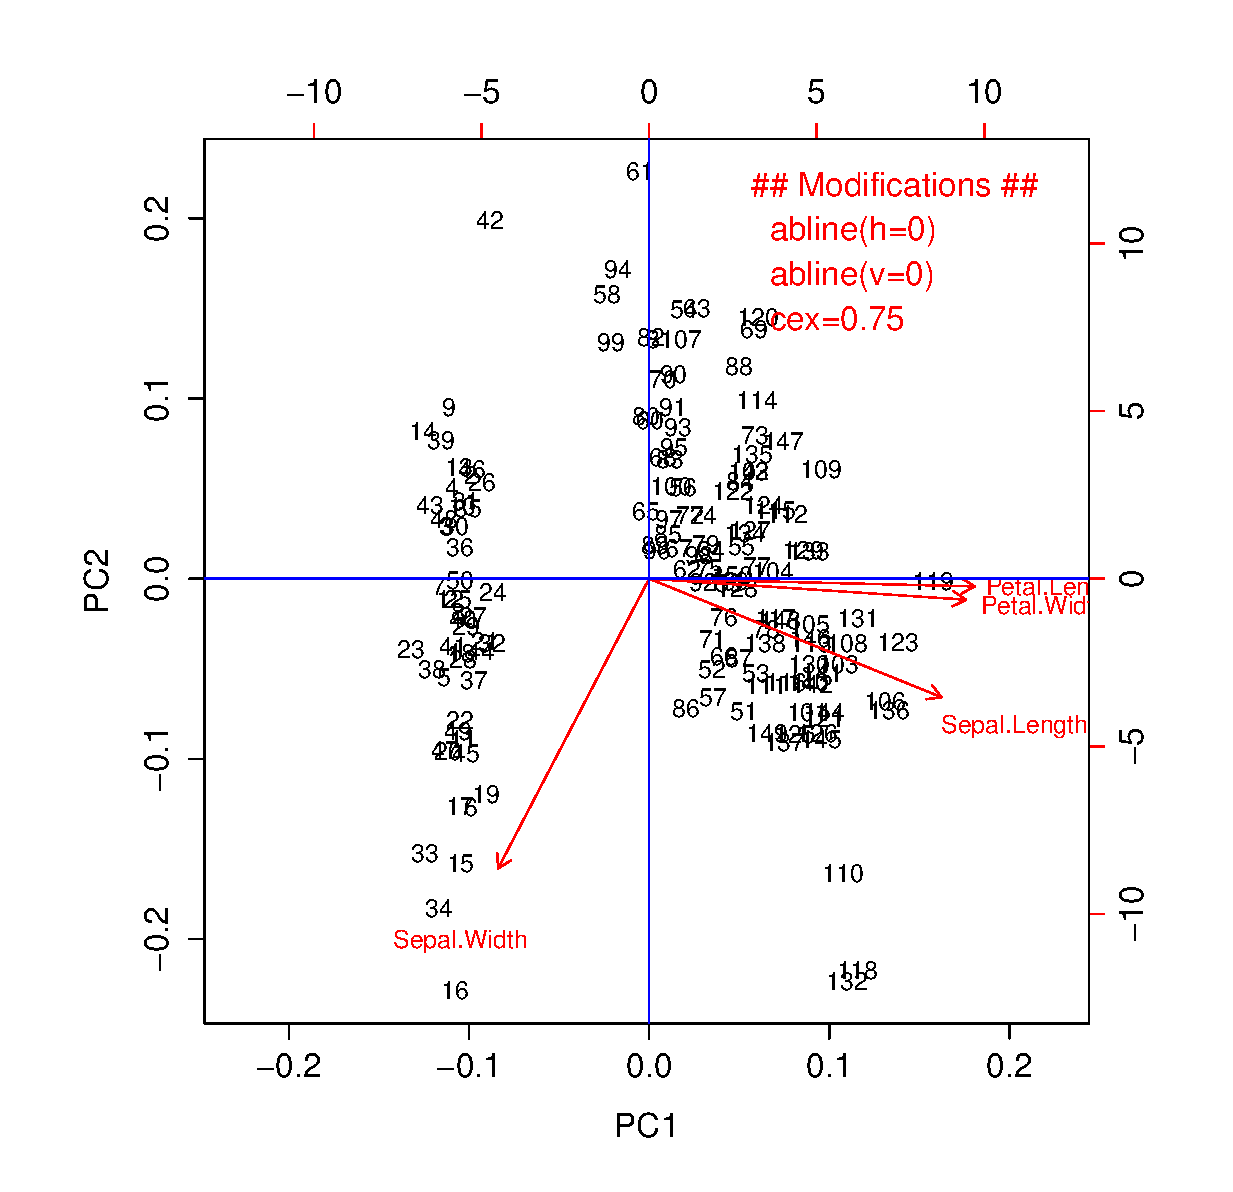
\includegraphics[clip]{./part4figures/irispca1.ps}}
%%%% NEW SIMPLER WAY TO SCALE, replace the above two lines with:
%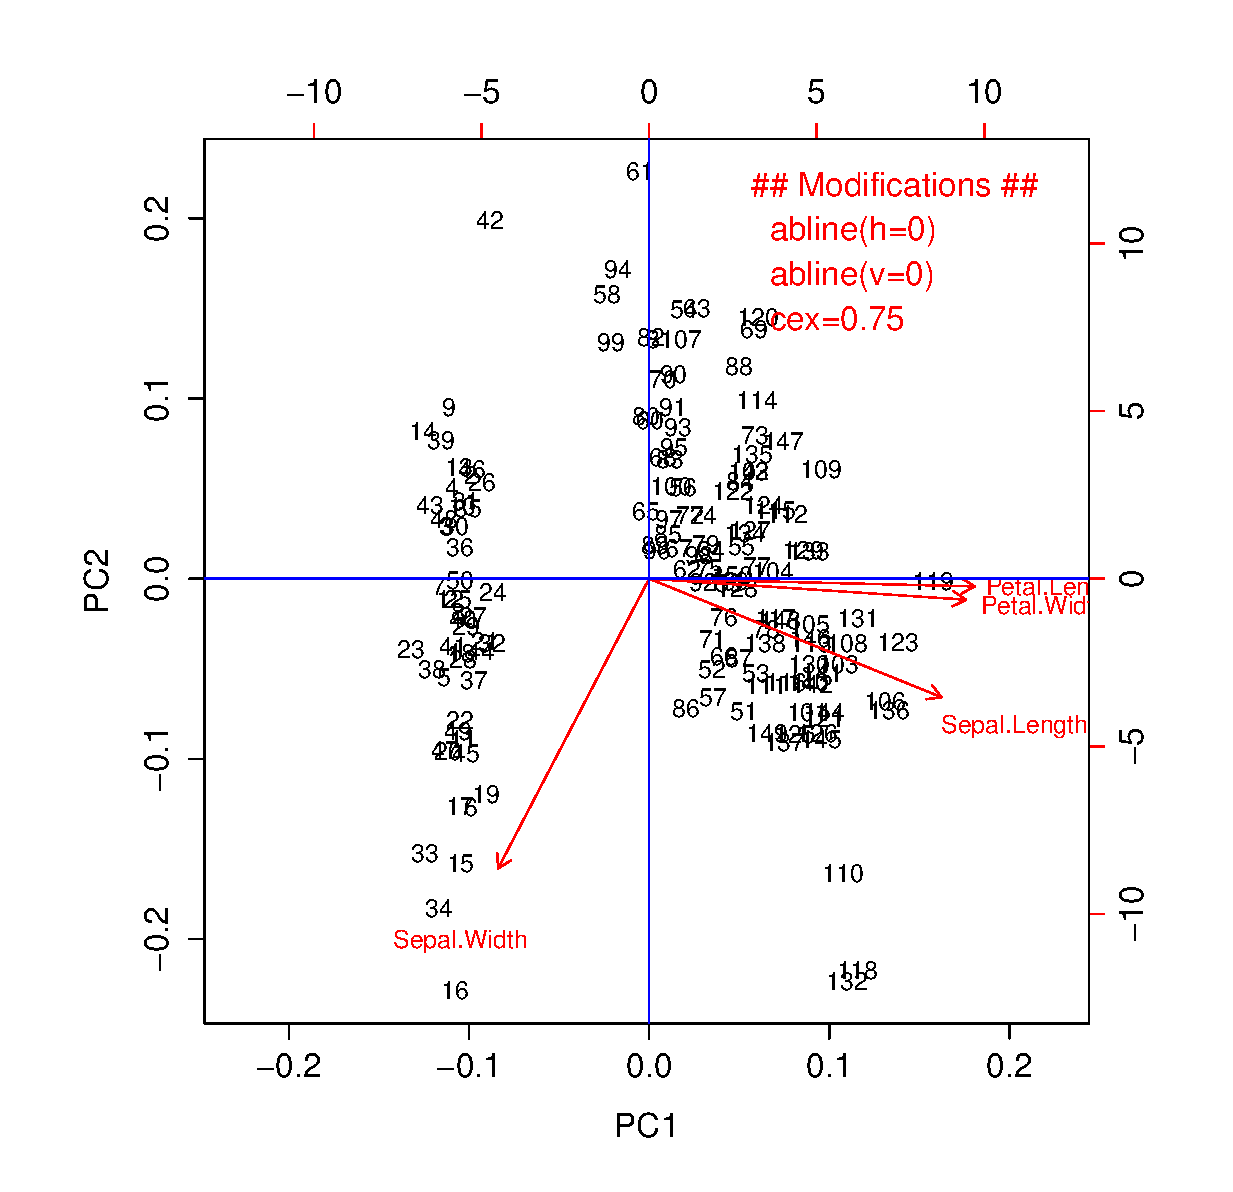
\includegraphics[clip,width=2.5in]{./part4figures/irispca1.ps}
\end{center}

%\vspace{-0.2in} 
{\scriptsize You can quickly examine sample and variable loading using the
  command {\color{red} \tt biplot(iris.prcomp)}.  The numbers
  indicate rows (iris samples) and the arrows show the 
  influence of each variable.\\}
\end{frame}


\begin{frame}[fragile]
\frametitle{Plotting PCA Results on a Scatterplot}

\bi
\item Scatterplots are a common way to show sample or variable
  ordinations (see Part 2 for help with {\color{red} \tt R} plotting syntax)

\item {\color{red} \tt plot(iris.prcomp\$x}) plots the first two
  principal components and is equivalent to {\color{red} \tt
    plot(iris.prcomp\$x[,c(1:2)])}

\item The following example uses several advanced plotting features to
  create a scatterplot of the samples on PC1 and PC2

{\scriptsize
\color{red}
\verb%op = par(mfrow=c(1,1))%\\
\verb%plot(iris.prcomp$x,%\\
\verb%  main="Principal Components Ordination of Iris Samples",%\\
\verb%  pch=c(21,22,24)[unclass(iris$Species)],%\\
\verb%  bg=c("pink", "violet", "purple")[unclass(iris$Species)],%\\
\verb%  cex=1.5)%\\
\verb%abline(h=0); abline(v=0)%\\
\verb%legend(x="topright", c("I. setosa", "I. versicolor", "I. virginica"),%\\
\verb%       pch=c(21, 22, 24), pt.bg=c("pink", "violet", "purple"),%\\
\verb%       bty="n", cex=1)%\\

\vspace{2ex}
\verb%#### To plot PC2 and PC3:%\\
\verb%plot(iris.prcomp$x[,c(2:3)])%\\

}
\ei

\end{frame}



\begin{frame}[fragile]
\frametitle{Scatterplot Showing PCA Sample Ordination}

\begin{center}
\resizebox{3in}{!}{
	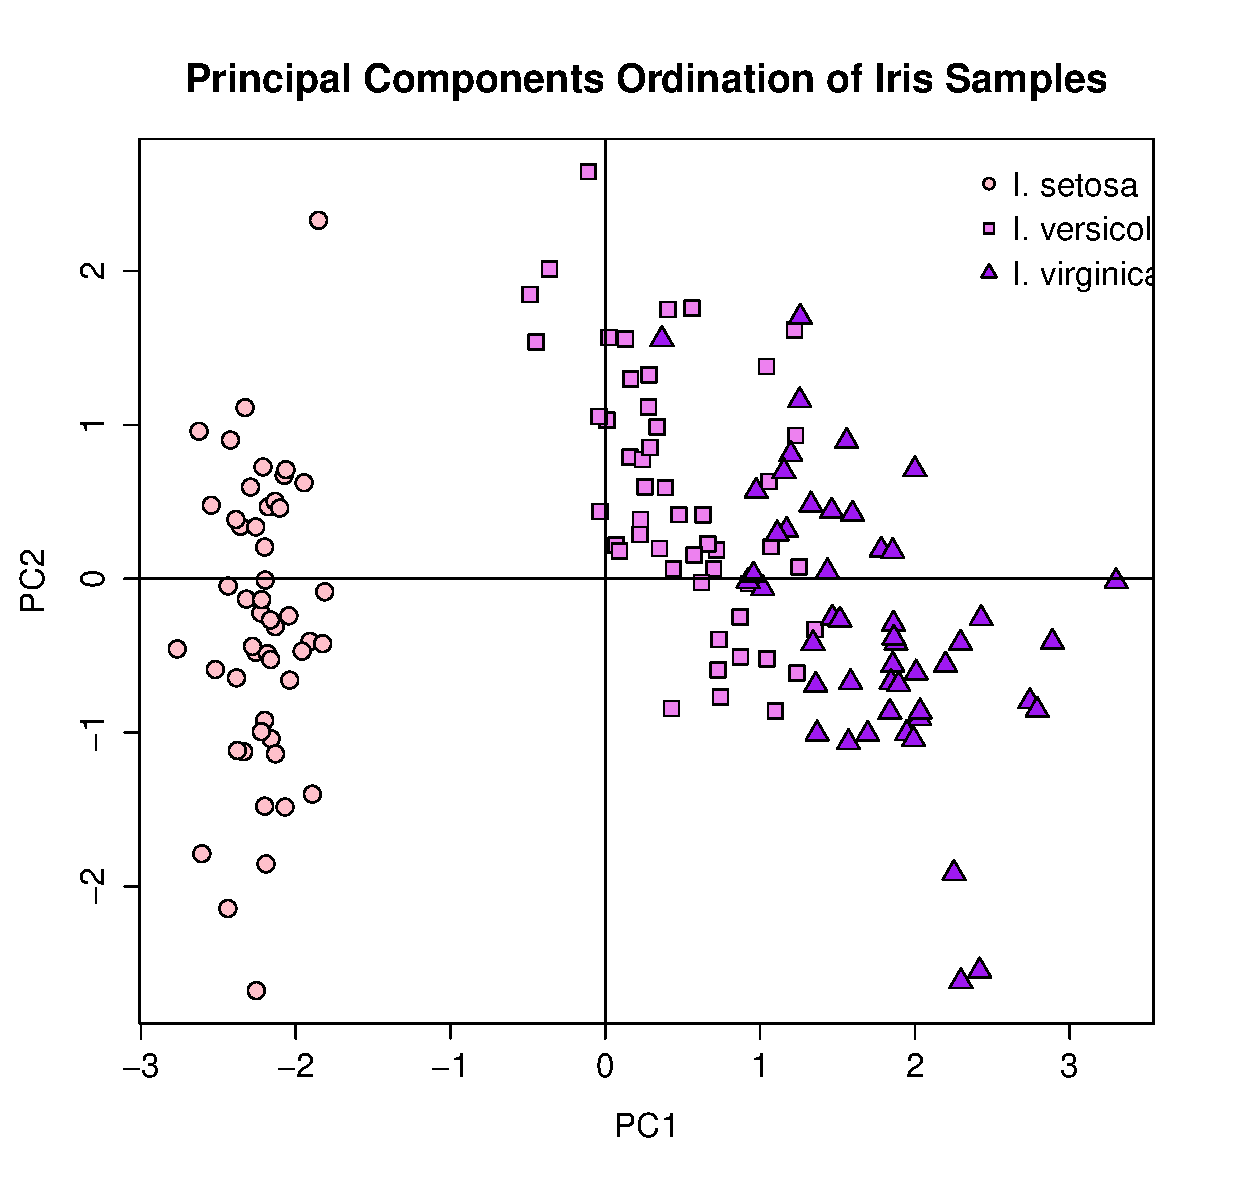
\includegraphics[clip]{./part4figures/irispca2.ps}}

\end{center}

\end{frame}


\begin{frame}
\frametitle{Multivariate Analysis - Clustering}
\framesubtitle{Hierarchical vs.~Divisive Clustering}

\bi
\item Most commonly used technique is {\color{blue}agglomerative,
hierarchical clustering}
	\bi
	\item Similarity (distance) is calculated between all samples
	\item The two closest samples (most similar) are combined into
          a joined sample containing all data from the two original
          samples
	\item The distances between all remaining samples and the
          joined sample are recalculated
	\item The next two closest samples are joined, and so on
	\ei
\item Another common technique is {\color{blue} divisive clustering},
where initial groups are defined, then all clusters are iteratively
regrouped until the with-in group distances are minimized
\ei 
\end{frame}


\begin{frame}
\frametitle{Multivariate Analysis - Clustering}
\framesubtitle{Interpreting Clustering Output}

\bi
\item Clustering is primarily an {\color{blue} exploratory} data analysis tool

\item Most clustering techniques are uninformed (you don't identify a grouping
  variable like site)

\bi
\item Divisive clustering requires that you specify the number of clusters to
  create, but the clusters are determined by similarity in the measured
  variables, not your definition of a group
\item This feature may identify groups you didn't expect or show you that
  your definition of a group is not correct
\ei

\item You can cluster random data $\ldots$ there is no automatic
significance test to prevent this from happening
	\bi
	\item You can test significance after clusters are identified
	\ei
\ei
\end{frame}


\begin{frame}
\frametitle{Hierarchical Clustering}
\framesubtitle{Measuring Distance Between Samples}

\bi
\item The first step in hierarchical clustering is to calculate
  the distance between samples ({\color{red} \tt dist})

\item Some of the distance methods available in {\tt \color{red} R} include

\vspace{2ex}
{\scriptsize
\begin{tabular}{lll}
Distance Method               & {\color{red} \tt R} Syntax           & Equation/Approach \\ \hline
Euclidean (Squared Euclidean) & {\color{red} \tt method="euclidean"} & $\sum{(x_{i} - y_{i})^{2}}$\\
Maximum (Chebychev)           & {\color{red} \tt method="maximum"}   & max$|x_{i} - y_{i}|$\\
Manhattan (City Block)        & {\color{red} \tt method="manhattan"} & $\sum{|x_{i} - y_{i}|}$\\
Canberra                      & {\color{red} \tt method="canberra"}  & $\sum{\frac{|x_{i} - y_{i}|}{|x_{i} + y_{i}|}}$\\
Binary                        & {\color{red} \tt method="binary"}    & count nonzero/zero \\ \hline
\end{tabular}
}

\vspace{2ex}
\item The default is {\color{red} \tt method="euclidean"}
\ei
\end{frame}


\begin{frame}
\frametitle{Hierarchical Clustering}
\framesubtitle{Example of Squared Euclidean Distance Calculations}

\begin{center}
\begin{tabular}{|l|ccc||lccc|} \hline
	& Var.~A	& Var.~B	& Var.~C		& \multicolumn{4}{||c|}{$X_{i} - Y_{i}$} \\ \hline
Site 1	& 20	& 10	& 17		& Site 1 -- Site 2: 	& 5		& 10		& 17\\
Site 2	& 15	& 0	& 0		& Site 1 -- Site 3:	& 20		& 4		& 17\\
Site 3	& 0	& 6	& 0		& Site 2 -- Site 3:	& 15		& --6		& 0\\ \hline
\end{tabular}
\end{center}


{\scriptsize
\begin{eqnarray*}
{\rm Distance\;}_{1-2} & = & (20-15)^{2} + (10-0)^{2} + (17-0)^{2} = (5^{2} + 10^{2} + 17^{2}) = 414\\
		&	& \\
{\rm Distance\;}_{1-3} & = & (20-0)^{2} + (10-6)^{2} + (17-0)^{2} = (20^{2} + 4^{2} + 17^{2}) = 705\\
		&	& \\
{\rm Distance\;}_{2-3} & = & (15-0)^{2} + (0-6)^{2} + (0-0)^{2} = (15^{2} + -6^{2} + 0^{2}) = 261
\end{eqnarray*}

\color{blue} Sites 2 and 3 are the closest based on squared Euclidean distance
}
\end{frame}



\begin{frame}
\frametitle{Hierarchical Clustering}
\framesubtitle{Measuring Distances Between Joined Samples (Cluster Method)}


\bi
\item The results from {\color{red} \tt dist} are used with
  {\color{red} \tt hclust} to complete the iterative clustering
  process

\item As with distance metrics, we can choose from a variety of
  clustering methods

\item The default method is the {\color{blue} farthest neighbor}
  (complete linkage), which joins groups using the two most distant members of each cluster.

\ei

\begin{center}
\resizebox{3in}{!}{
	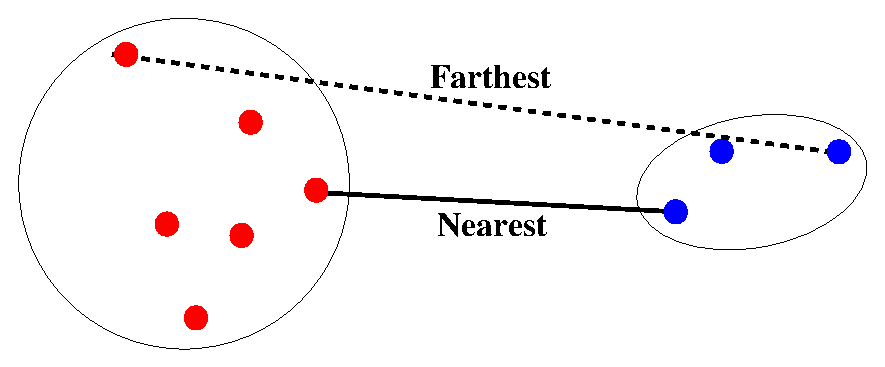
\includegraphics{./part4figures/neighbors.eps}}

\end{center}
\end{frame}


\begin{frame}
\frametitle{Hierarchical Clustering}
\framesubtitle{Other Clustering Methods - Average Distance}

{\footnotesize Average distance (unweighted pair group method with
  arithmetic mean; UPGMA) gives equal weight to each sample in the
  cluster\\}

{\tiny
\begin{eqnarray*}
d(A,D) & = & \sqrt{(4-15)^{2} + (11-8)^{2}} = 11.4018\\
	&  & \\
d(A,E) & = & \sqrt{(4-16)^{2} + (11-9)^{2}} = 12.1655
\end{eqnarray*}
}

\vspace{-0.5in}
\begin{center}
\resizebox{3in}{!}{
	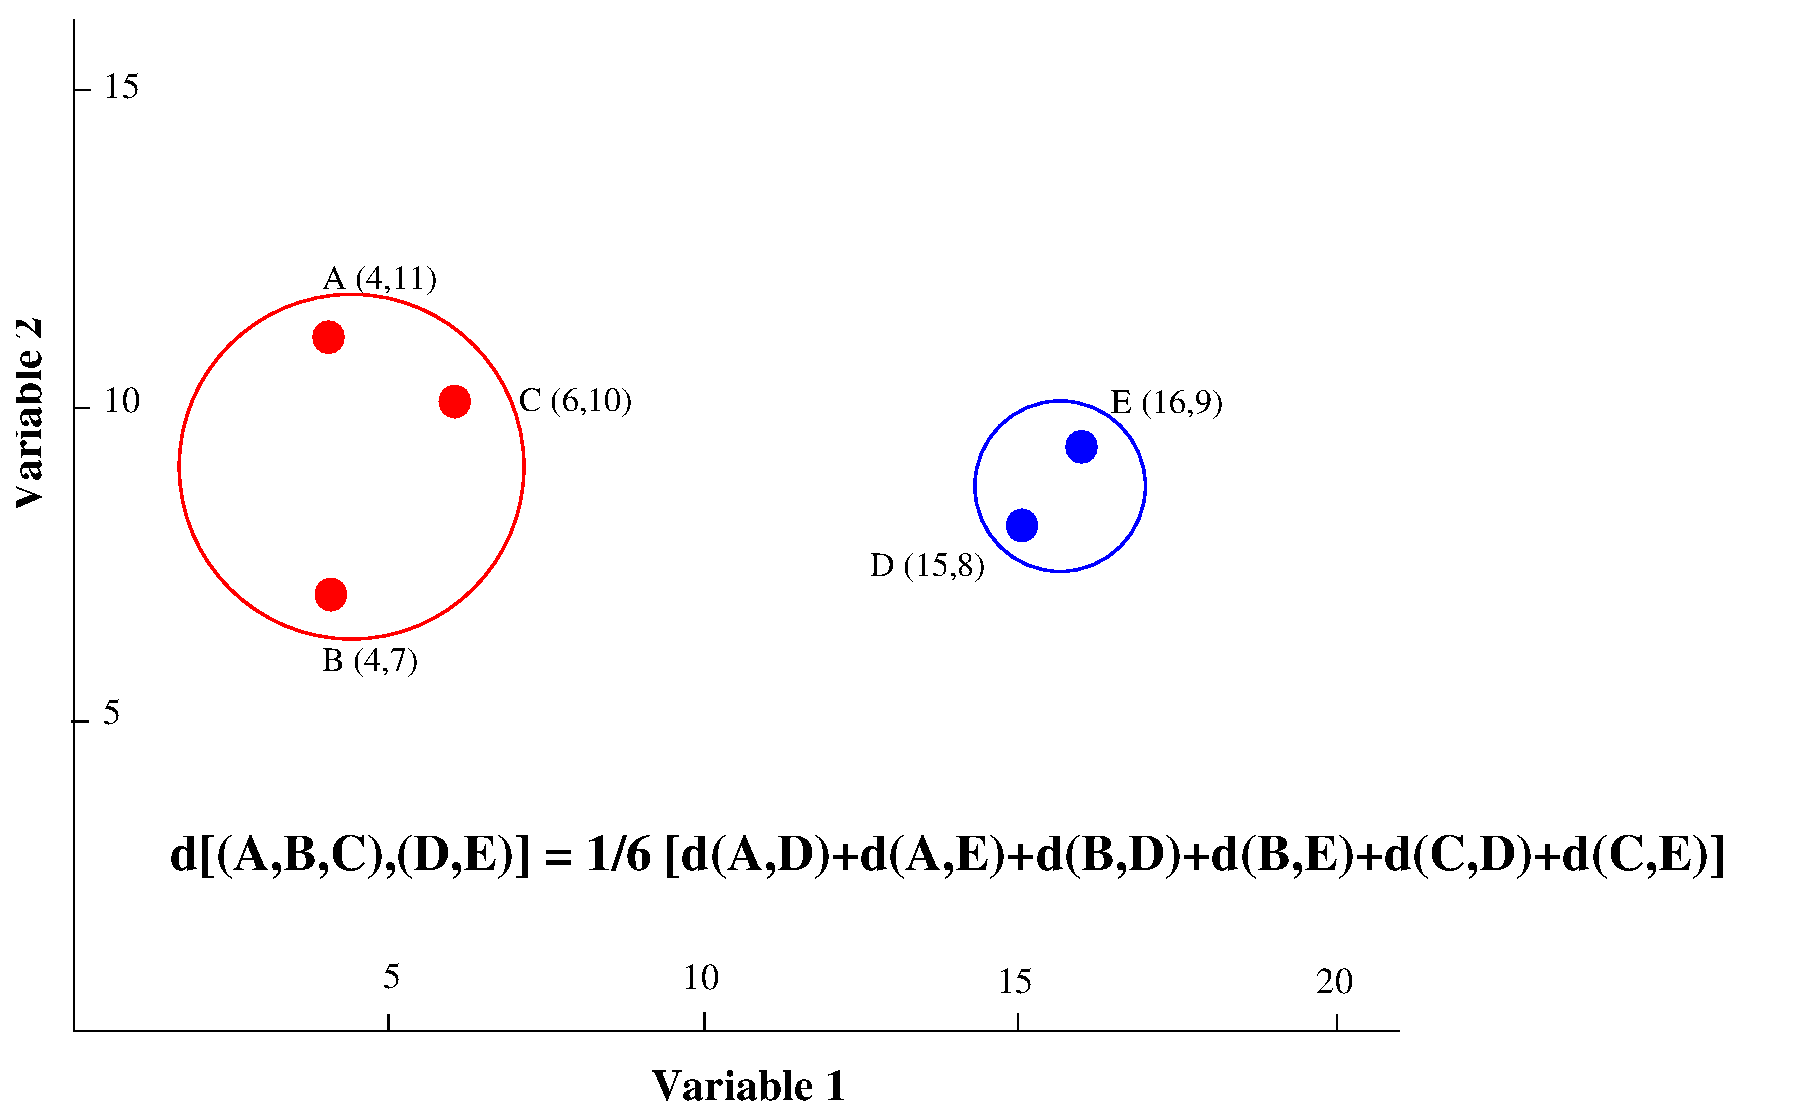
\includegraphics{./part4figures/upgma.eps}}
\end{center}

\end{frame}

\begin{frame}
\frametitle{Hierarchical Clustering}
\framesubtitle{Other Clustering Methods - Wards Minimum Variance}

\bi
\item {\em Ward's minimum variance} often produces different results

\item After each cluster cycle, the sample pairs with the lowest
  within-cluster sums of squares is joined next

\item This approach preserves groups with small internal variance
\ei

\begin{center}
\resizebox{3in}{!}{
	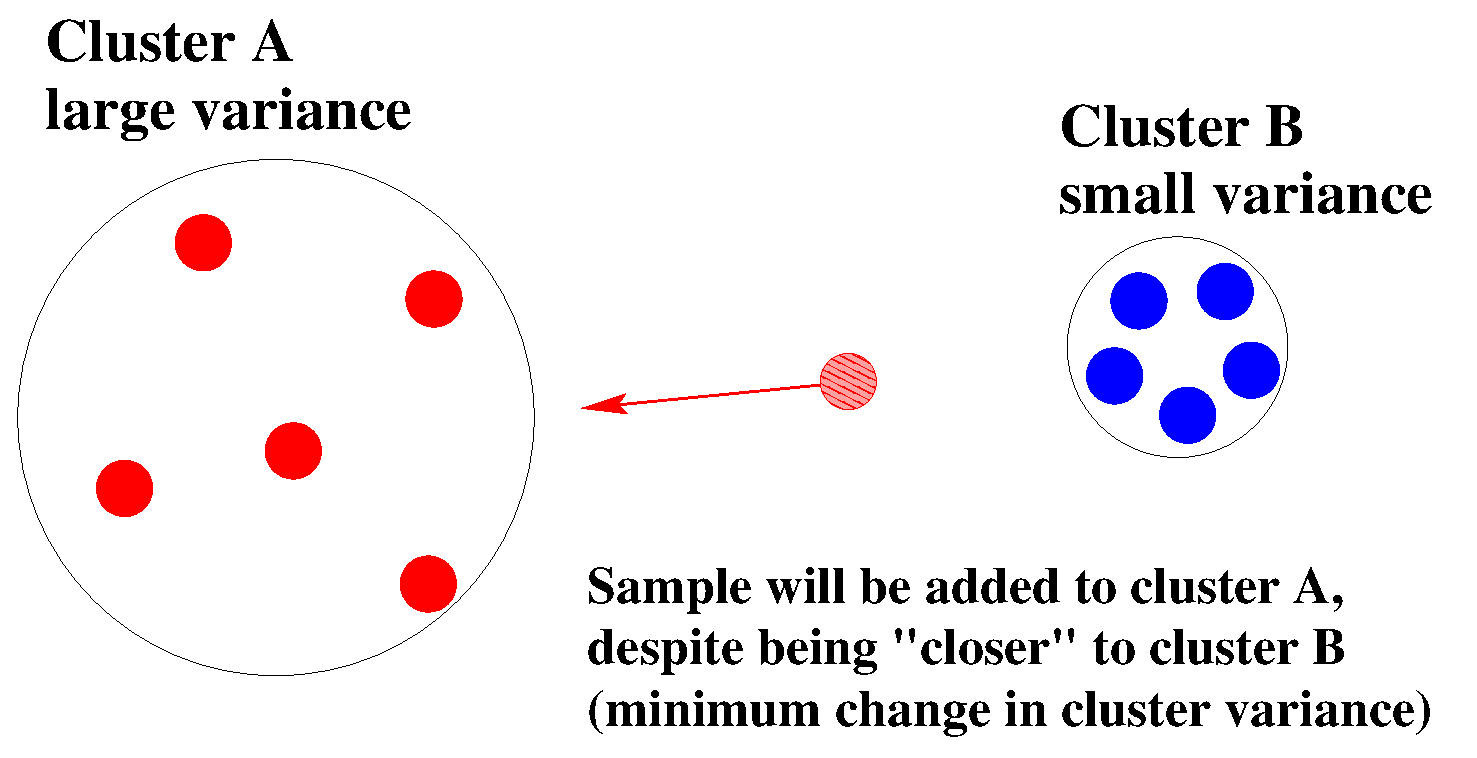
\includegraphics{./part4figures/minvar.eps}}
\end{center}

\end{frame}


\begin{frame}[fragile]
\frametitle{Clustering of First 10 Rows For Each Iris Species}


{\scriptsize
\color{red}
\verb%### First example - Euclidean distance with farthest neighbor:%\\
\verb%data(iris); attach(iris)%\\

\vspace{2ex}
\verb%### Step 1:  select data subset and distance metric%\\
\verb%edist <- dist(iris[c(1:10, 51:60, 101:110), c(1:4)],%\\
\verb%        method="euclidean")%\\

\vspace{2ex}
\verb%### Step 2: select clustering method%\\
\verb%edist.complete <- hclust(edist, method="complete")%\\

\vspace{2ex}
\verb%### Step 3: plot the results as an edited dendrogram%\\
\verb%plot(edist.complete, labels=iris[c(1:10, 51:60, 101:110), 5],%\\
\verb%     ylab="Euclidean Distance", xlab=" ", main=" ", sub=" ")%\\

\vspace{4ex}
\verb%### Second example - Euclidean distance with Ward's minimum variance%\\

\vspace{2ex}
\verb%edist.ward <- hclust(edist, method="ward")%\\

\vspace{2ex}
\verb%### Add hang=-1 to place samples on x-axis%\\
\verb%plot(edist.ward, labels=iris[c(1:10, 51:60, 101:110), 5],%\\
\verb%     ylab="Euclidean Distance", xlab=" ", main=" ", sub=" ", hang=-1)%\\
}

\end{frame}


\begin{frame}[fragile]
\frametitle{Euclidean Distance/Farthest Neighbor}
\label{iriscluster1}
\begin{center}
\resizebox{3in}{!}{
	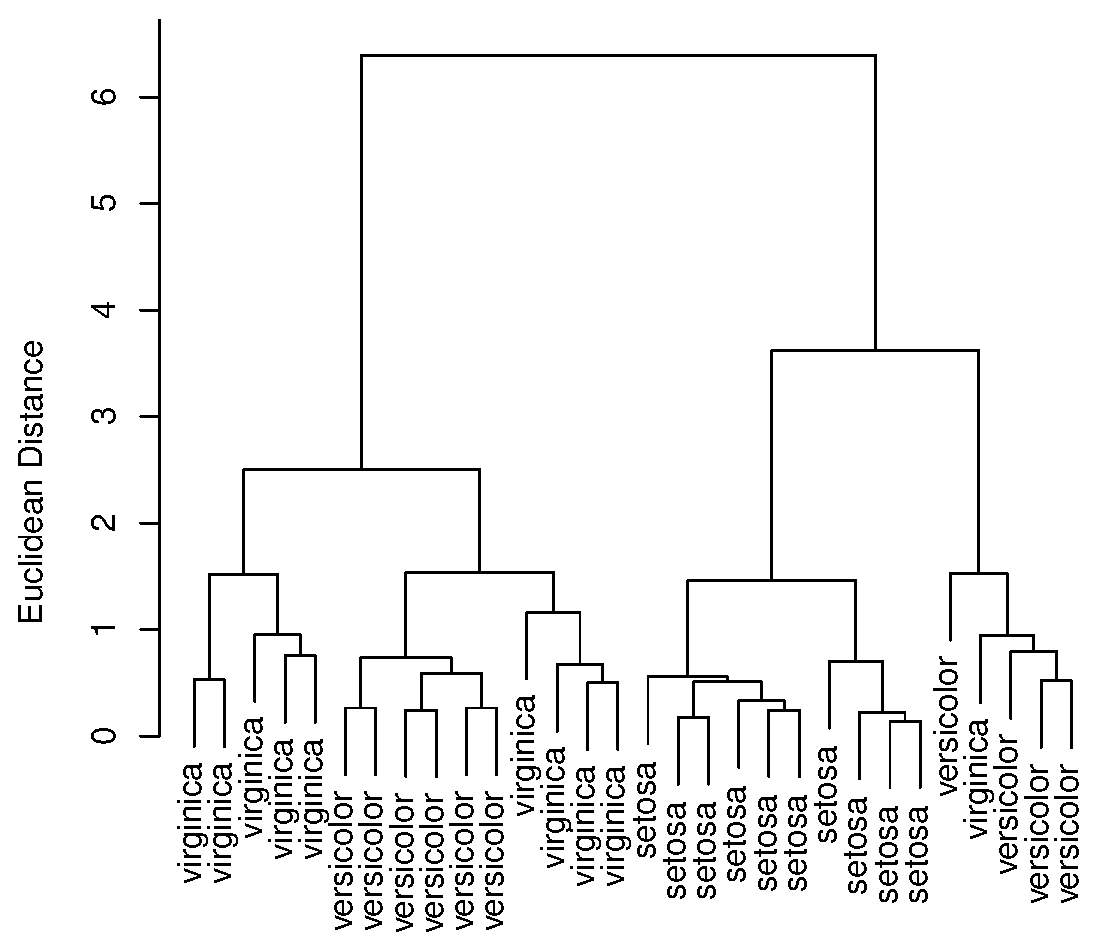
\includegraphics{./part4figures/iriscluster1a.eps}}
\end{center}
\end{frame}

\begin{frame}[fragile]
\frametitle{Euclidean Distance/Farthest Neighbor}
\begin{center}
\resizebox{3in}{!}{
	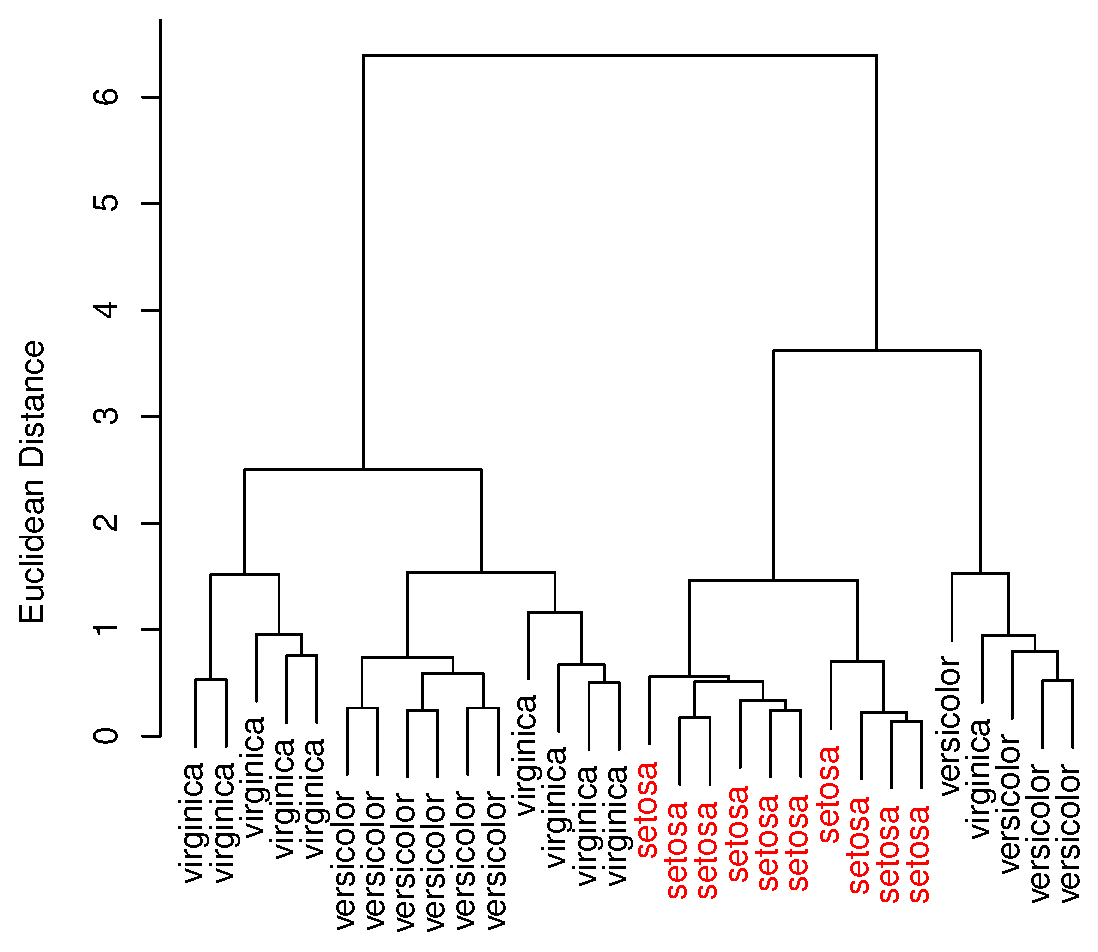
\includegraphics{./part4figures/iriscluster1b.eps}}
\end{center}
\end{frame}


\begin{frame}[fragile]
\frametitle{Euclidean Distance/Ward's Minimum Variance}
\label{iriscluster2}
\begin{center}
\resizebox{3in}{!}{
	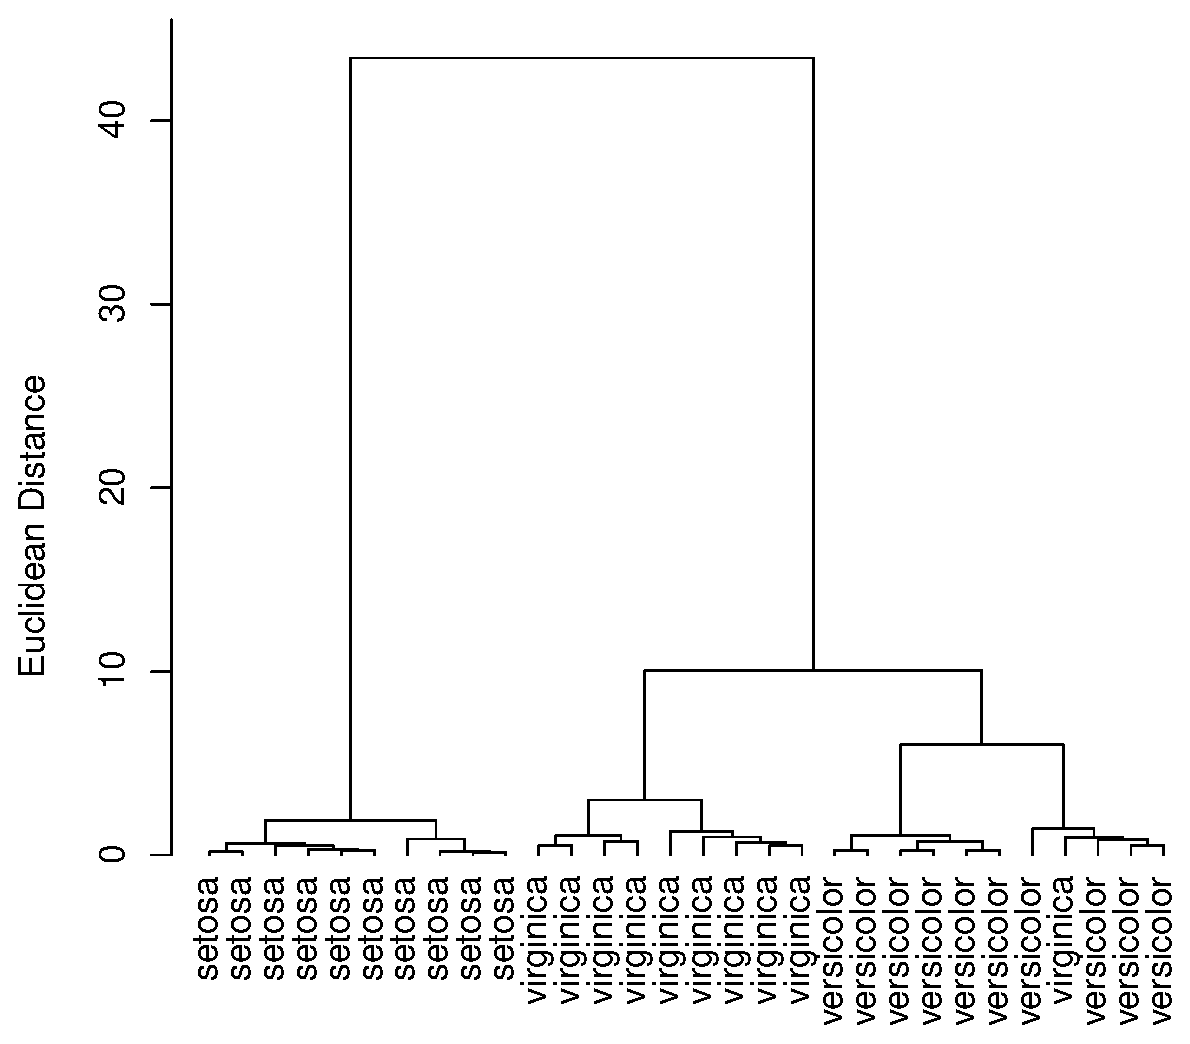
\includegraphics{./part4figures/iriscluster2a.eps}}
\end{center}

\end{frame}

\begin{frame}[fragile]
\frametitle{Euclidean Distance/Ward's Minimum Variance}
\begin{center}
\resizebox{3in}{!}{
	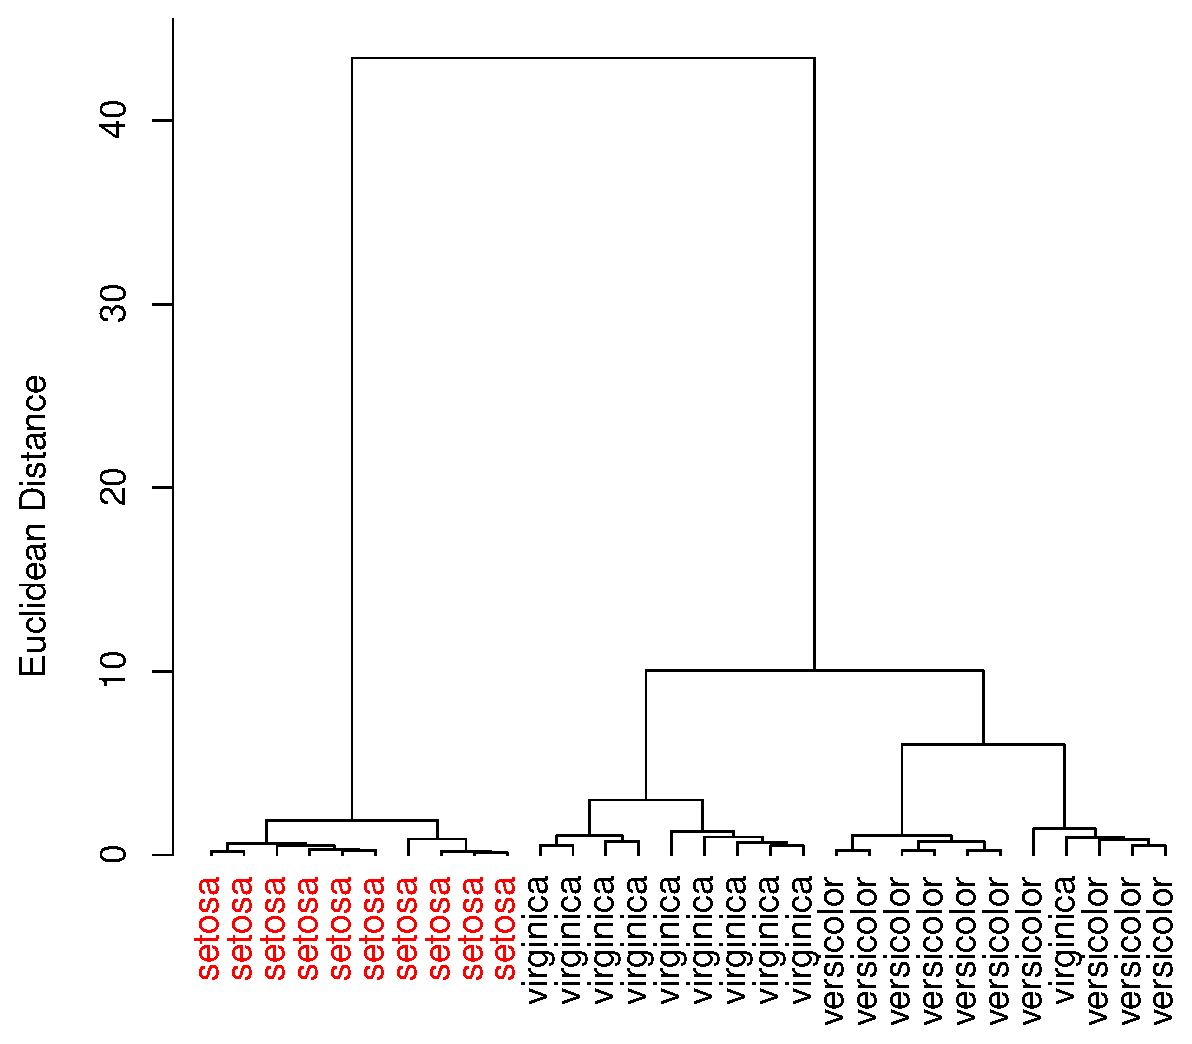
\includegraphics{./part4figures/iriscluster2b.eps}}
\end{center}

\end{frame}

\begin{frame}[fragile]
\frametitle{Euclidean Distance/Ward's Minimum Variance}
\begin{center}
\resizebox{3in}{!}{
	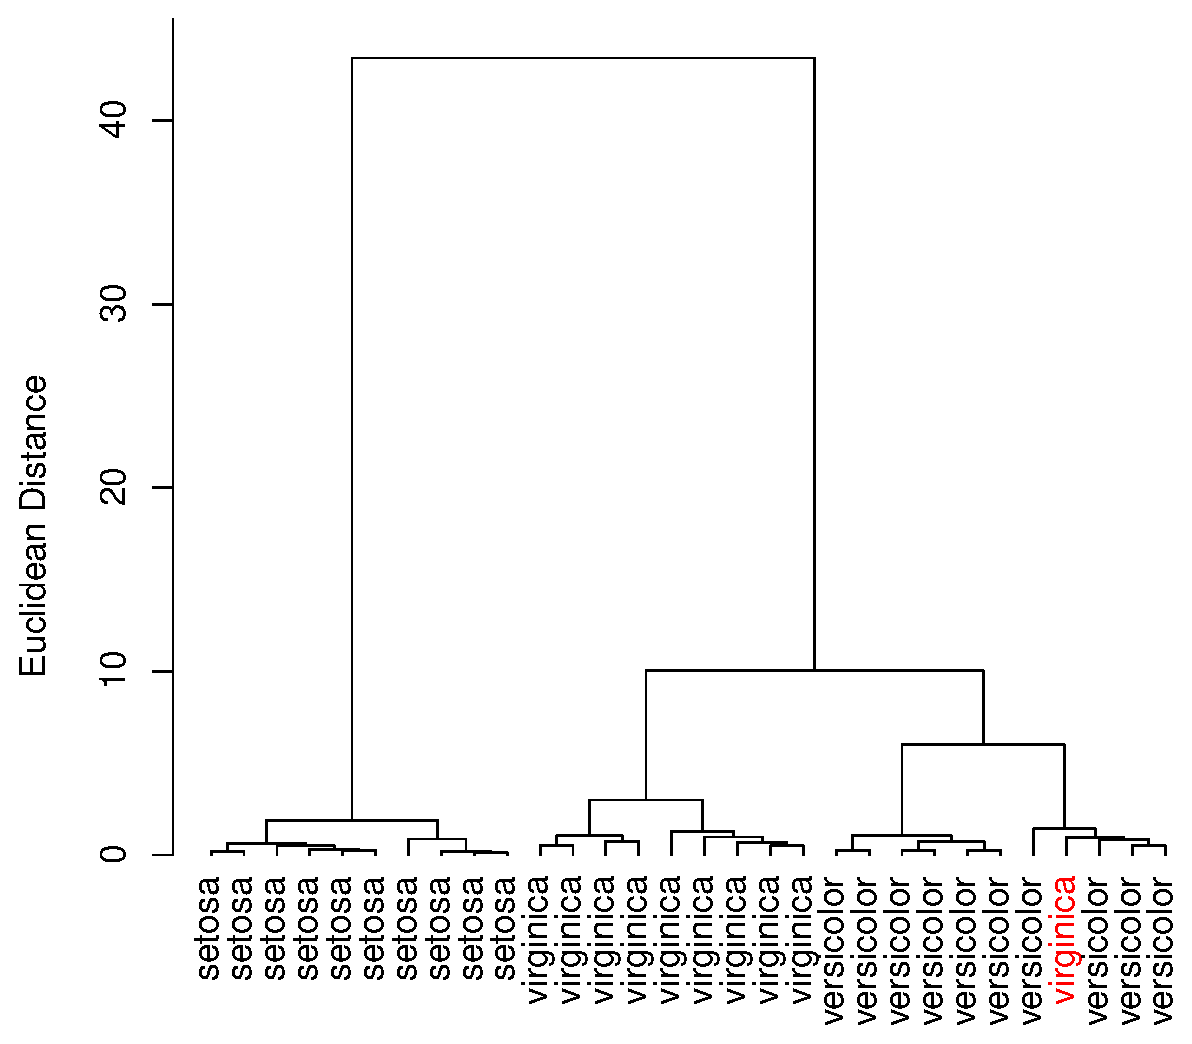
\includegraphics{./part4figures/iriscluster2c.eps}}
\end{center}
\end{frame}


\begin{frame}
\frametitle{Multivariate Analysis - Divisive Clustering}
\framesubtitle{KMeans Clustering of Fisher's Iris Data (n=30)}

\bi
\item KMeans clustering starts with {\color{blue} {\em n} centers} for each variable
\item Distances are computed to all points simultaneously

\item The center is moved and distances recomputed, with the objective
of minimizing distance (measured as within groups sums of squares)

\item The {\tt \color{red}R} program lets you set the number of iterations
or times the centers are moved.  The default is 10 iterations  
	\bi
	\item More iterations take time, but produce a more repeatable result
	\ei

\item Because the cluster centers are based on iterations, repeated
k-means clustering can produce different results.  
\ei
\end{frame}


\begin{frame}[fragile]
\frametitle{Divisive Clustering - Iris Data}
\framesubtitle{{\tt \color{red} R} Syntax for KMeans Clustering into Three Groups}

KMeans clustering produces the number of groups you request. In this
example, we ask for 3 groups to match our assumption that each of the
3 species will cluster separately

\vspace{2ex}
{\scriptsize
\color{red}

\verb%irispart <- iris[c(1:10, 51:60, 101:110),] # R shortcut!%\\
\verb%kcluster3 <- kmeans(irispart[ , c(1:4)], 3)%\\
\verb%kcluster3  #This produces the cluster summary%\\

\vspace{2ex}
\color{blue}
\verb%### Edited output:%\\
\verb%Cluster means:%\\
\verb%  Sepal.Length Sepal.Width Petal.Length Petal.Width%\\
\verb%1        4.860       3.310     1.450000        0.22%\\
\verb%2        6.875       3.025     6.012500        2.10%\\
\verb%3        5.975       2.825     4.441667        1.45%\\

\vspace{2ex}
\verb%Clustering vector:%\\
\verb%  1   2   3   4   5   6   7   8   9  10  51  52  53  54  55  56  57  58  59  60 %\\
\verb%  1   1   1   1   1   1   1   1   1   1   3   3   3   3   3   3   3   3   3   3 %\\
\verb%101 102 103 104 105 106 107 108 109 110 %\\
\verb%  2   3   2   2   2   2   3   2   2   2 %\\
}
\end{frame}



%%% highlighted output:
\begin{frame}[fragile]
\frametitle{Divisive Clustering - Iris Data}
\framesubtitle{{\tt \color{red} R} Syntax for KMeans Clustering into Three Groups}

{\small \color{red}

\vspace{1ex}
\color{blue}
\verb%### Edited output:%\\
\verb%Cluster means:%\\
\verb%  Sepal.Length Sepal.Width Petal.Length Petal.Width%\\
\color{blue}\verb%1        4.860       3.310% \color{red}\verb%     1.450000        0.22%\\
\color{blue}\verb%2        6.875       3.025% \color{red}\verb%     6.012500        2.10%\\
\color{blue}\verb%3        5.975       2.825% \color{red}\verb%     4.441667        1.45%\\

\color{blue}
\vspace{1ex}
\verb%Clustering vector:%\\
\verb%  1   2   3   4   5   6   7   8   9  10%\\ 
\verb%  1   1   1   1   1   1   1   1   1   1   ### All setosa in Group 1%\\

\vspace{1ex}
\verb%51  52  53  54  55  56  57  58  59  60 %\\
\verb%3   3   3   3   3   3   3   3   3   3     ### All versicolor in Group 3%\\

\vspace{1ex}
\verb%101 102 103 104 105 106 107 108 109 110 %\\
\verb%  2   3   2   2   2   2   3   2   2   2   ### 8 virginica in Group 2%\\
\vspace{3ex}
\verb%### Misclassification rate:  2/30 = 6.7 pct %\\
}
\end{frame}


\begin{frame}[fragile]
\frametitle{Divisive Clustering - Iris Data}
\framesubtitle{Scatterplot Matrix Showing KMeans 3-Group Clusters}
\begin{center}
\resizebox{2.5in}{!}{
	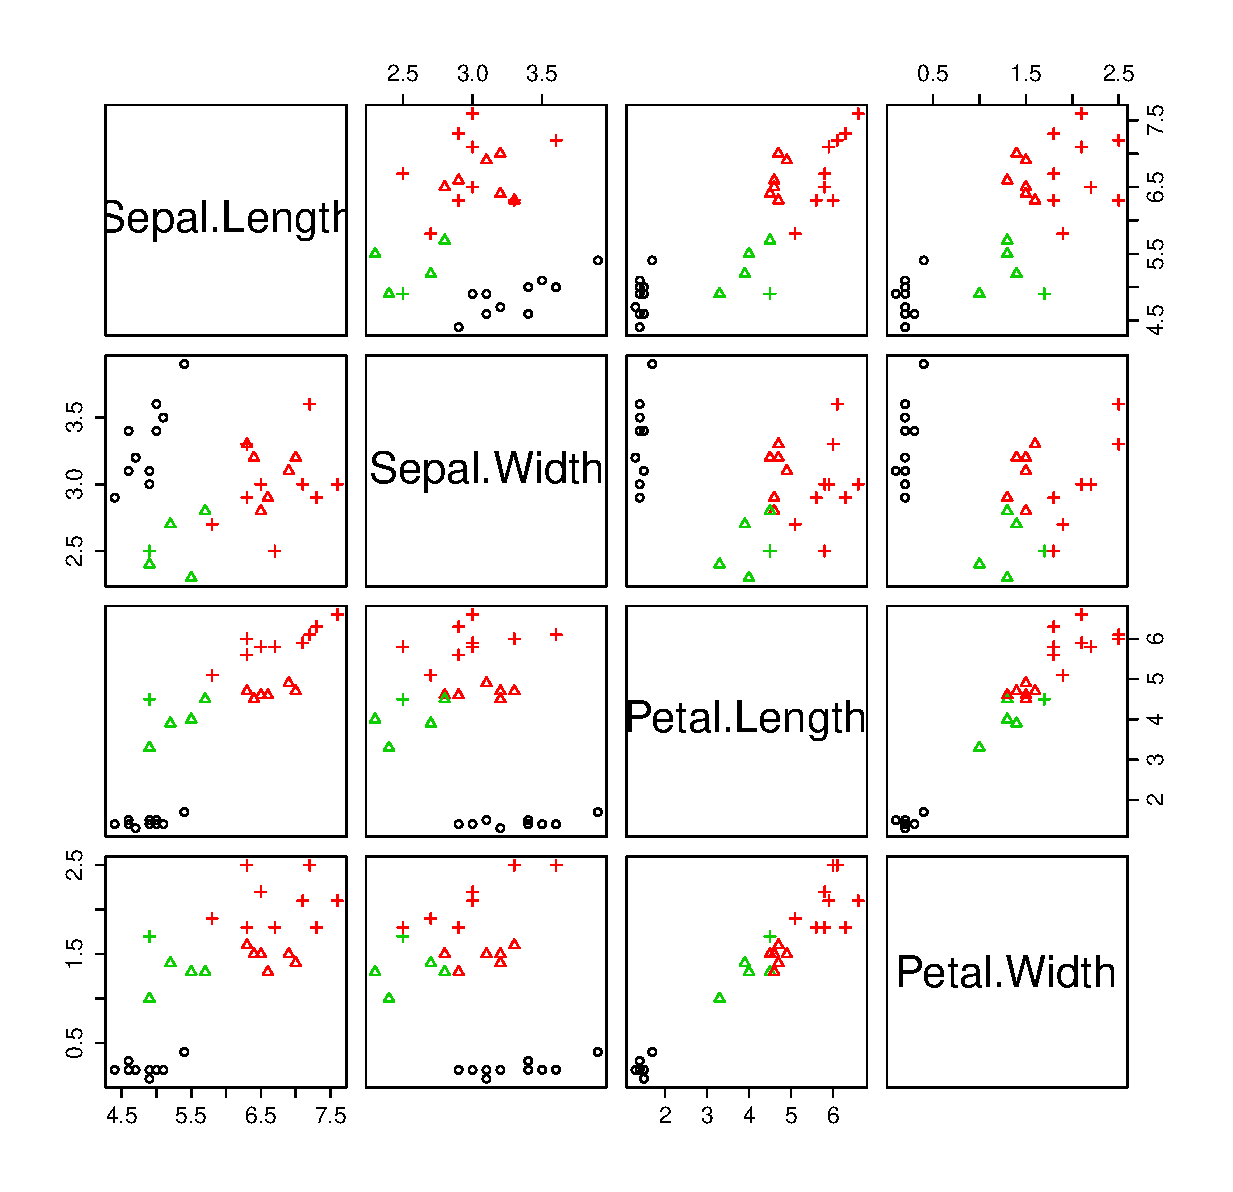
\includegraphics[clip]{./part4figures/iriscluster3.ps}}
\end{center}

\vspace{-3ex}
{\scriptsize \color{red}
\verb%plot(irispart[, c(1:4)], col=kcluster3$cluster, pch=unclass(irispart[,5]))%\\
}

\end{frame}


\begin{frame}[fragile]
\frametitle{Divisive Clustering - Iris Data}
\framesubtitle{Plotting Results Using Best Two Variables; Adding Association Analysis}
{\scriptsize 
\color{red}
\verb%data(iris); attach(iris)%\\
\verb%kcluster3.all <- kmeans(iris[, c(1:4)], 3)%\\
\verb%table(Species, kcluster3.all$cluster)%\\
           
\color{blue}
\verb%Species       1  2  3%\\
\verb%  setosa     50  0  0%\\
\verb%  versicolor  0  2 48%\\
\verb%  virginica   0 36 14%\\

\vspace{2ex}
\color{red}
\verb%chisq.test(Species, kcluster3.all$cluster)%\\

\color{blue}
\verb%	Pearson's Chi-squared test%\\
\verb%data:  Species and kcluster3.all$cluster %\\
\verb%X-squared = 223.5993, df = 4, p-value < 2.2e-16%\\

\vspace{3ex}
\color{red}
\verb%plot(Petal.Length, Petal.Width, %\\
\verb%     pch=c(21, 22, 24)[unclass(Species)],%\\
\verb%     cex=1.7, xlab="Petal Length (cm)", ylab="Petal Width (cm)",%\\
\verb%     main="Kmeans Clustering of Iris Data Into Three Groups",%\\
\verb%     bg=c("pink", "violet", "purple")[kcluster3.all$cluster])%\\
\verb%legend(x="topleft", c("I. setosa", "I. versicolor", "I. virginica"), %\\
\verb%       pch=c(21, 22, 24), bty="n")%\\
\verb%legend(x="top", c("Group 1", "Group 2", "Group 3"), %\\
\verb%       fill=c("pink", "violet", "purple"), bty="n")%\\
\verb%legend(x="bottomright", c("misclassification = 10.7 pct",%\\
\verb%       "(2 versicolor + 14 virginica)"), bty="n")%\\
}

\end{frame}


\begin{frame}
\frametitle{Divisive Clustering - Iris Data}
\framesubtitle{Plotting Results Using Best Two Variables; Adding Association Analysis}
\begin{center}
%\resizebox{3in}{!}{
%	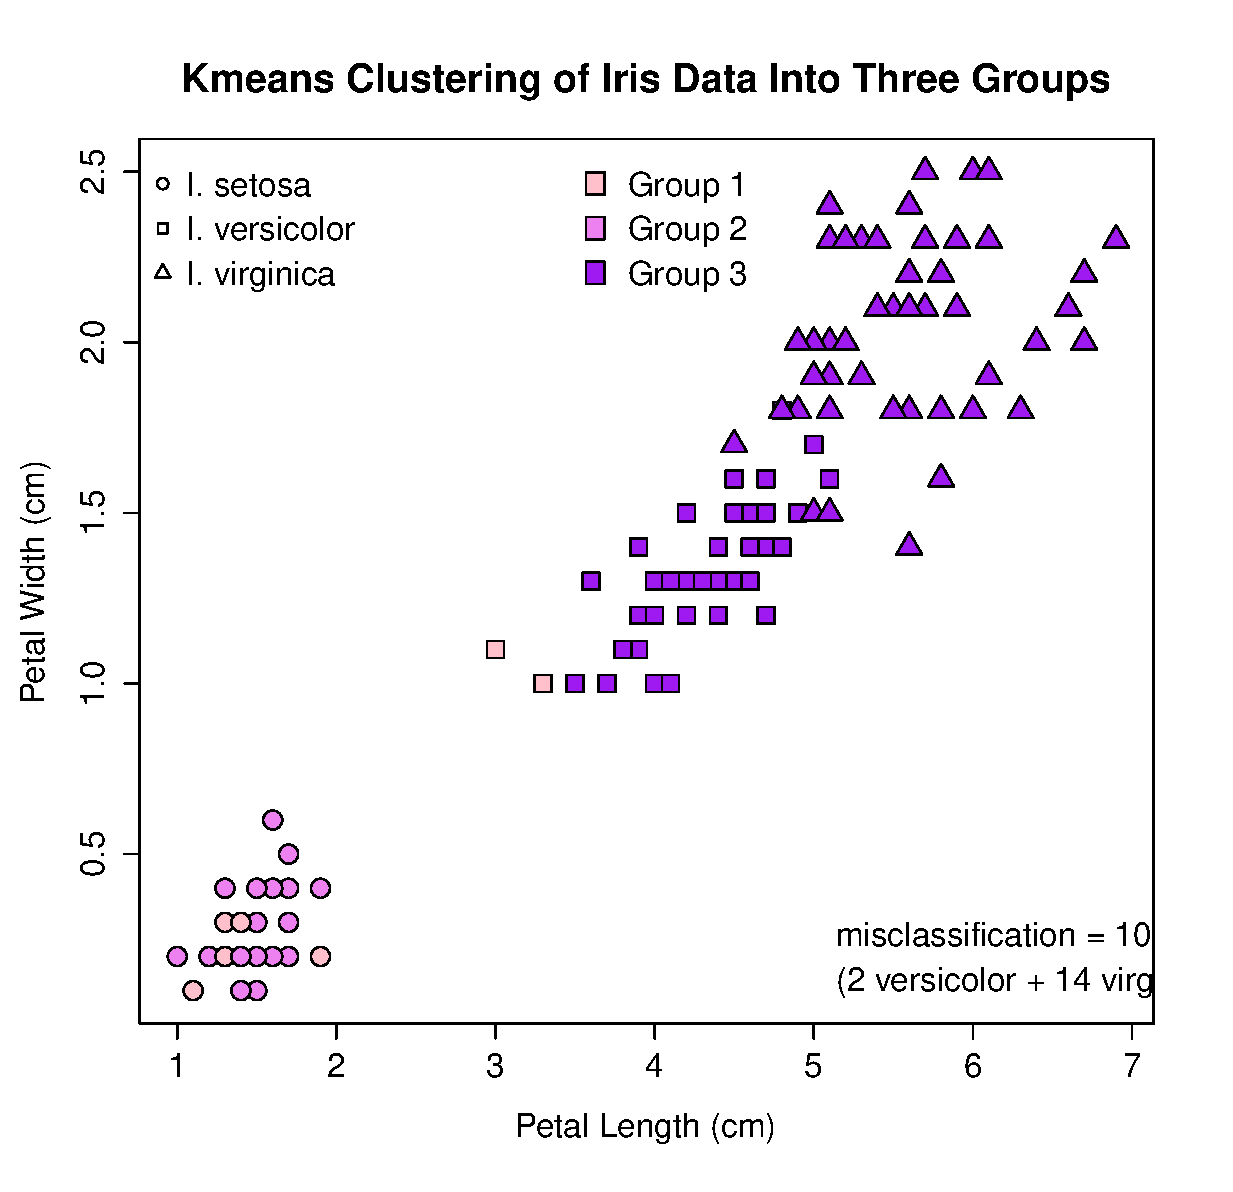
\includegraphics[clip]{./part4figures/iriscluster4.ps}}
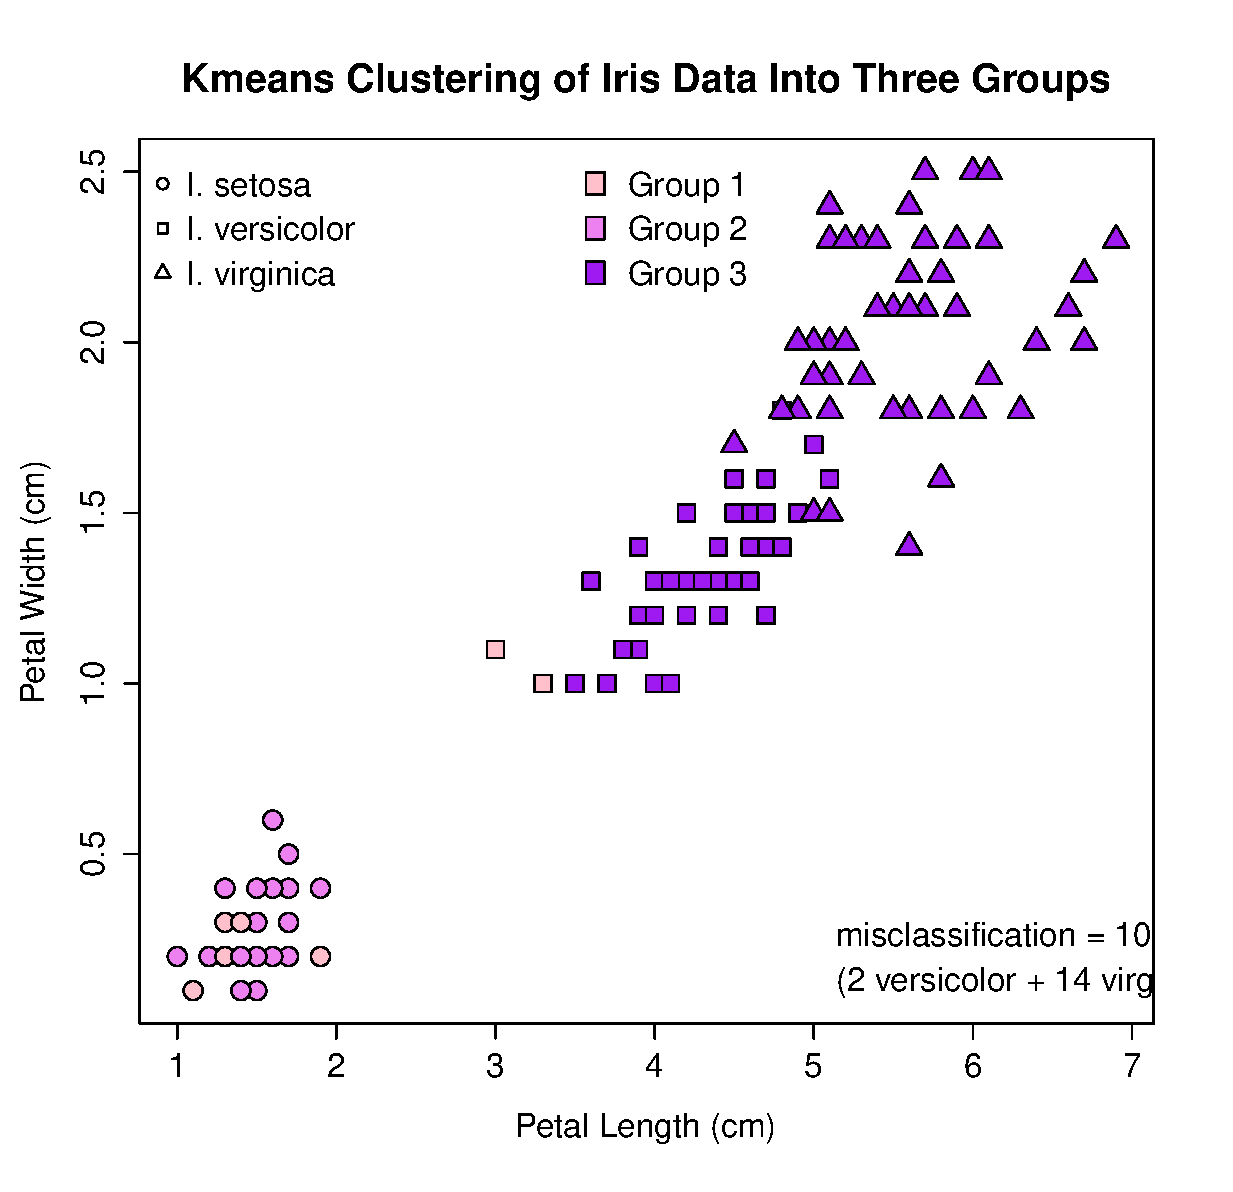
\includegraphics[clip,width=3in]{./part4figures/iriscluster4.ps}
\end{center}
\end{frame}




\begin{frame}[fragile]
\frametitle{Advanced Topics - Clustering on Principal Components}
\framesubtitle{Microcosm Test Using Contaminated Sediments}

\bi
\item This example published by Chariton, et al.~(2014) following the
  approach described by Ben-Hur and Guyon (2003)

\item Data are from a sediment toxicity test to determine the effects
  of zero/low/high concentrations of triclosan (antibiotic/antifungal
  compound) on sediment biota

\item Sediment biota were identified using pres/abs molecular markers
  that identified $>$850 {\em different} sediment organisms
\item The biota were listed by {\em operational taxonomic units}
  (OTUs) rather than genus and species (OTUs)
\ei
\end{frame}


\begin{frame}[fragile]
\frametitle{Clustering on Principal Components}
\framesubtitle{Preliminary Data Decisions}

\bi
\item The source file contained presence/absence data for 858 OTUs
  from three treatments (control, low, high) with six replicates per
  treatment

\item Nine OTUs were excluded because they had identical values for
  all samples (variance = zero)

\item Final data set contained 18 rows and 849 variables (OTUs)

\item The data were analyzed using scaled {\color{red} \tt
    prcomp}

\item PCA truncated at 18 components (residual variance $<$3.3e-15)
  \ei
\end{frame}



\begin{frame}[fragile]
\frametitle{Clustering on Principal Components}
\framesubtitle{Step 1:  Creating New Variables from Component Scores}

{\scriptsize 
\color{red}
\verb%#### create the PCA using OTUs (col 1-2 = treatment/replicate)%\\
\verb%alldata <- read.csv("alldataOTU.csv", T); attach(alldata)%\\
\verb%alldataPCA <- prcomp(alldata[, c(3:851)], scale=T)%\\
\verb%summary(alldataPCA)%\\

\vspace{2ex}
\color{blue}
\verb%Importance of components:%\\
\verb%                          PC1   PC2     PC3     PC4    PC5     PC6     PC7%\\
\verb%Standard deviation     10.221 9.880 8.77070 8.08297 7.7312 7.28034 7.03630%\\
\verb%Proportion of Variance  0.123 0.115 0.09061 0.07695 0.0704 0.06243 0.05832%\\
\verb%Cumulative Proportion   0.123 0.238 0.32863 0.40559 0.4760 0.53842 0.59673%\\
\verb%                           PC8     PC9    PC10   PC11    PC12    PC13    PC14%\\
\verb%Standard deviation     6.75020 6.71040 6.52041 6.3837 6.27286 5.86208 5.52219%\\
\verb%Proportion of Variance 0.05367 0.05304 0.05008 0.0480 0.04635 0.04048 0.03592%\\
\verb%Cumulative Proportion  0.65040 0.70344 0.75352 0.8015 0.84786 0.88834 0.92426%\\
\verb%                          PC15    PC16    PC17      PC18%\\
\verb%Standard deviation     5.05834 4.56602 4.22722 3.321e-15%\\
\verb%Proportion of Variance 0.03014 0.02456 0.02105 0.000e+00%\\
\verb%Cumulative Proportion  0.95440 0.97895 1.00000 1.000e+00%\\

\vspace{2ex}
\color{red}
\verb%#### write the scores to a new data set:%\\
\verb%PCA.scores <- data.frame(alldata$treatment, alldata$replicate, round(alldataPCA$x, 3))%\\
\verb%write.table(PCA.scores, "alldataPCA.csv", quote=F, row.names=F, col.names=T, sep=",")%\\
}
\end{frame}


\begin{frame}[fragile]
\frametitle{Clustering on Principal Components}
\framesubtitle{Variance Plot for First 10 Components}

\begin{center}
\resizebox{3in}{!}{
	\includegraphics{./part4figures/pca3_new/PCAvariableplot.ps}}

{\scriptsize \color{red}
\vspace{-0.5in}
\verb%plot(alldataPCA, col=rainbow(10), main=" ")%\\
}
\end{center}
\end{frame}



\begin{frame}[fragile]
\frametitle{Clustering on Principal Components}
\framesubtitle{Comparison of Original and New Data Sets}


\begin{center}
{\scriptsize
\begin{tabular}{ccccc}
\multicolumn{5}{c}{\bf Original Sediment Microcosm Data (18 rows, 851 columns)}\\
\multicolumn{5}{c}{ }\\
Treatment & Replicate & OTU 1  & $\ldots$ & OTU 849\\\hline
control   & 1         & 0 or 1   &        & 0 or 1\\
control   & 2         & 0 or 1   &        & 0 or 1\\
(etc.)    & (etc.)    & (etc.)   &        & (etc.) \\      
high      & 5         & 0 or 1   &        & 0 or 1\\
high      & 6         & 0 or 1   &        & 0 or 1\\\hline
\end{tabular}

\vspace{8ex}

\begin{tabular}{ccccc}
\multicolumn{5}{c}{\bf PCA Data - {\color{red} \tt alldataPCA\$x} (18 rows, 20 columns) - }\\
\multicolumn{5}{c}{ }\\
Treatment & Replicate & PC 1      & $\ldots$ & PC 18\\ \hline
control   & 1         & -4.97    &        & $<$ $\pm$0.01\\
control   & 2         & -15.53   &        & $<$ $\pm$0.01\\
(etc.)    & (etc.)    & (etc.)   &        & (etc.) \\      
high      & 5         & 13.81    &        & $<$ $\pm$0.01\\
high      & 6         & 13.10    &        & $<$ $\pm$0.01\\\hline
\end{tabular}


}
\end{center}

\end{frame}


\begin{frame}[fragile]
\frametitle{Clustering on Principal Components}
\framesubtitle{Step 2:  Clustering on the Component Scores}

\bi
\item The next process is based on the fact that the scaled, centered
  PCA creates a multivariate correlation matrix, with the ``best''
  correlations contained in the first component

\item Each successive component containing a smaller fraction of
  ``good'' correlation

\item We want to cluster using the smallest subset of components that
  will produce stable clusters $\ldots$ this is a significant
  departure from traditional ordination

\item The next figure shows initial euclidean/wards hierarchical clustering
  using all 18 principal components as a starting point
\ei
\end{frame}


\begin{frame}[fragile]
\frametitle{Clustering on Principal Components}
\framesubtitle{Dendrogram Results using 18 Components}

\begin{center}
\resizebox{2.5in}{!}{
	\includegraphics{./part4figures/pca3_new/hclustPCAall.ps}}
\end{center}

{\scriptsize
\vspace{-0.4in}
\color{red}
\verb%newdata <- read.csv("alldataPCA.csv", T); attach(newdata)%\\
\verb%distances <- dist(newdata[, c(3:20)], method="euclidean")%\\
\verb%eward <- hclust(distances, method="ward")%\\
\verb%plot(eward, labels=treatment, hang=0, cex=0.65, xlab=" ", sub=" ",%\\
\verb%      main="PC1-18 (100%)", ylab="Euclidean Distance")%\\
\\}
\end{frame}


\begin{frame}[fragile]
\frametitle{Clustering on Principal Components}
\framesubtitle{Step 3: Identifying Stable Clusters}

\bi
\item Selecting the fewest components for stable clustering is actually
  a complex process (see Ben-Hur and Guyon, 2003)

\item Preliminary evaluation of the 18-component clusters reveal that
  there are only two {\em treatment} responses (high vs.~control$+$low)

\item Using {\color{red} \tt cuttree} and {\color{red} \tt table}, we
  can look at the number of misclassifications between the cluster
  groups and treatment, with misclassification defined as samples that
  don't match ``high'' or ``control$+$low

\item Cycling through all dendrograms, (PC1--PC18, PC1--PC17,
  PC1--PC16, etc), each results in 1 misclassification until the final
  option (PC1--PC2), which results in 2 misclassifications

{\color{blue} \em You only need PC1--PC3 to produce
  stable clusters}
\ei

\end{frame}


\begin{frame}[fragile]
\frametitle{Clustering on Principal Components}
\framesubtitle{Dendrogram Results using First Seven Principal Components}

\begin{center}
%\includegraphics[height=\textheight]{./part4figures/pca3_new/hclustPCAsubset.ps}
\resizebox{4in}{2.8in}{
	\includegraphics{./part4figures/pca3_new/hclustPCAsubset.ps}}
\end{center}

\end{frame}


\begin{frame}[fragile]
\frametitle{Clustering on Principal Components}
\framesubtitle{Step 4: Refining Cluster Membership and Checking Significance}

\bi
\item After selecting the minimum number of components for clustering,
  we should review cluster membership

\item The figure on page 41 %\pageref{pcacluster1} 
shows how two PCA cluster
  groups match ``high'' and ``low$+$control'' treatments, with one
  misclassification

\item But the figure on page 42 %\pageref{pcacluster2} 
reveals that you
  could also describe the data using three clusters

\bi
\item Two of the clusters show treatment
  effects (high or low$+$control)
\item The third cluster contains three outlier samples
\ei

\item Choosing which way to display the results depends on your
  overall goals, but it is usually desirable to discuss outliers
  separately from the treatment effect
\ei

\end{frame}


\begin{frame}[fragile]
\frametitle{Clustering on Principal Components}
\framesubtitle{Two-Cluster Dendrogram}
\label{pcacluster1}

\begin{center}
\resizebox{4in}{2.5in}{
	\includegraphics{./part4figures/pca3_new/hclustPCAbest.ps}}
\end{center}

\vspace*{-5ex}
{\scriptsize \color{red}
\verb%HCgroups <- cutree(eward, 2); chisq.test(HCgroups, treatment)%\\

\color{blue}
\verb%X-squared = 13.8462, df = 2, p-value = 0.0009848%\\
}
\end{frame}


\begin{frame}[fragile]
\frametitle{Clustering on Principal Components}
\framesubtitle{Three-Cluster Dendrogram}
\label{pcacluster2}

\begin{center}
\resizebox{4in}{2.5in}{
	\includegraphics{./part4figures/pca3_new/hclustPCAbest3.ps}}
\end{center}

\vspace*{-5ex}
{\scriptsize \color{red}
\verb%HCgroups <- cutree(eward, 3); chisq.test(HCgroups, treatment)%\\

\color{blue}
\verb%X-squared = 17.6, df = 4, p-value = 0.001477%\\
}
\end{frame}


\begin{frame}[fragile]
\frametitle{Clustering on Principal Components}
\framesubtitle{Step 5: Interpreting the Results}

\bi
\item Using this approach, the data revealed two treatment
  responses (not three) and a subgroup of outliers from different treatment groups

\item To finish the evaluation, we can examine how the source data
  influenced the principal components

\item With continuous data (e.g., water quality, algae counts), you
  could use summary statistics (e.g., minimum, median, maximum) for
  each cluster group

\item Summary statistics are not helpful for presence/absence data, so
  we examined the top 10 negative and positive OTU scores for the PC1--PC3 
  ({\color{red} \tt alldataPCA\$rotation}; table on page
  \pageref{otuscores}) \ei
\end{frame}

\begin{frame}[fragile]
\label{otuscores}
{\scriptsize
\begin{center}
\begin{tabular}{lc|lc|lc}
\multicolumn{6}{c}{\bf Best Negative Variable Scores in PC1-PC3}\\
OTU	& PC1	  & OTU 	& PC2	        & OTU 	        & PC3\\ \hline
M.5324	& -0.085  & M.521	& -0.087	& M.33548	& -0.082\\
M.18385	& -0.083  & F.671	& -0.087	& M.29634	& -0.076\\
M.17875	& -0.083  & uk.euk.3152	& -0.087	& uk.euk.29604	& -0.074\\
M.34715	& -0.083  & S.3978	& -0.087	& M.10729	& -0.074\\
M.25065	& -0.082  & S.7008	& -0.087	& M.4300	& -0.073\\
M.28527	& -0.082  & M.7687	& -0.087	& R.848	        & -0.071\\
uk.euk.6428 & -0.082 & S.9894	& -0.087	& uk.euk.6422	& -0.071 \\
M.1091	& -0.081  & S.10341	& -0.087	& S.947	        & -0.071\\
M.15718	& -0.080  & S.13318	& -0.087	& uk.euk.11428	& -0.071\\
M.25537	& -0.079  & S.15201	& -0.087	& uk.euk.4378	& -0.071\\ \hline
\multicolumn{6}{l}{ }\\					
\multicolumn{6}{l}{ }\\					
\multicolumn{6}{c}{\bf Best Positive Variable Scores in PC1-PC3}\\
OTU	& PC1	  & OTU 	& PC2	        & OTU 	        & PC3\\ \hline
R.1633	& 0.056	& F.35789	& 0.037	& M.20011	& 0.075\\
M.37505	& 0.056	& uk.euk.28316	& 0.037	& R.27994	& 0.075\\
R.28351	& 0.056	& M.588	        & 0.038	& A.25541	& 0.075\\
M.37021	& 0.057	& M.25299	& 0.039	& M.29451	& 0.075\\
M.37060	& 0.060	& uk.euk.35868	& 0.040	& M.26907	& 0.075\\
S.3563	& 0.065	& M.10534	& 0.040	& M.35148	& 0.076\\
R.9197	& 0.066	& M.15282	& 0.041	& M.35761	& 0.080\\
Am.5381	& 0.068	& S.37132	& 0.044	& uk.euk.8723	& 0.081\\
A.11234	& 0.073	& M.4361	& 0.048	& uk.euk.4435	& 0.084\\
R.30870	& 0.077	& M.5776	& 0.052	& uk.euk.5340	& 0.088\\\hline
\end{tabular}
\end{center}
}
\end{frame}



\begin{frame}[fragile]
\frametitle{Plotting the Samples by PCA Scores}

\begin{center}
\resizebox{4.5in}{2.5in}{
	\includegraphics{./part4figures/pca3_new/PCAsampleplot.ps}}

{\scriptsize 
PC1 separated the two treatment groups; PC2 and PC3 were useful for separating
  the outliers\\
}
\end{center}

\end{frame}



\begin{frame}
\frametitle{Supplemental References}

\bi
\item Crawley, Michael J.  2013.  The R Book.  John Wiley \&
  Sons. ISBN 978-0-470-97392-9.

\item Everitt, Brian S.  2011.  Cluster Analysis, 5th Edition.
Wiley, ISBN 978-0-470-74991-3.
 
\item Lander, Jared P.  2014.  R for Everyone, Advanced Analytics and
  Graphics.  Addison Wesley Data \& Analytics Series, ISBN
  978-0-321-88803-7.

\item Pielou, Evelyn C.  1984.  The Interpretation of Ecological Data:
  A Primer on Classification and Ordination. Wiley.
  978-0-471-88950-2.

\item Teetor, Paul. 2011.  The R Cookbook.  O'Reilly Publishers. ISBN
  978-0-596-880915-7 
\ei
\end{frame}

\begin{frame}
\frametitle{Citations for PCA Clustering}

\bi
\item Ben-Hur, A.~and I.~Guyon.  2003.  Detecting stable clusters
  using principal component analysis in methods in molecular biology.
  In Brownstein, M.~J.~and A.~Kohodursky, eds, {\em Functional
    Genomics: Methods and Protocols.}, Humana Press, Totowa, NJ, pp
  159--182.

\item Chariton, A.~A., K.~T.~Ho, D.~Proestou, H.~Bik, S.~L.~Simpson,
  L.~M.~Portis, M.~G.~Cantwell, J.~G.~Baguley, R.~M.~Burgess,
  M.~M.~Pelletier, M.~Perron, C.~Gunsch, and R.~A.~Matthews.  2014.  A
  molecular-based approach for examining responses of eukaryotes in
  microcosms to contaminant-spiked estuarine sediments.  {\em
    Environmental Toxicology and Chemistry} 33:359--369.
\ei
\end{frame}

\end{document}
\end
